\section*{Problem 1}
	\begin{enumerate} [a)]
		\item 
		\begin{proof} [Solution]
			Use the variables: \texttt{Total population} = 30, \texttt{initial infected} = 1, \texttt{day} = 150, \texttt{speed} = 0.01, \texttt{recovery} = 25, \texttt{distance} = 0.03.
			\begin{center}
				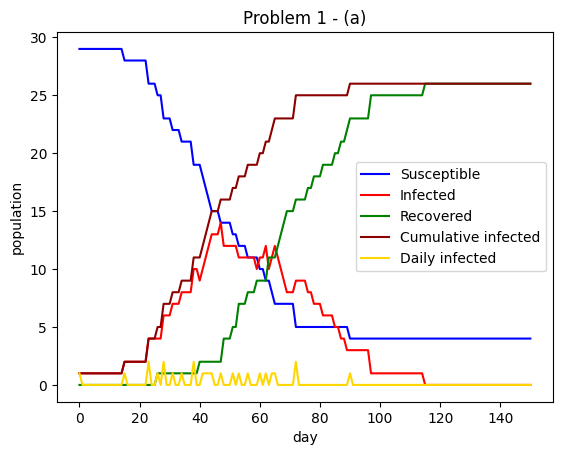
\includegraphics[scale=0.7]{Problem1_a.png}
			\end{center}
		\end{proof}
		\item 
		\begin{proof} [Solution]
			Control the 3 variables: \texttt{speed}, \texttt{recovery}, and \texttt{distance}. Before running the model, we can expect the behavior of each population.
			\begin{itemize}
				\item If \texttt{speed} increases, then the chances of infected people coming into contact with susceptible increases. Additionally, as the distance traveled per day increases, the number of infected can increase significantly in an instant.
				\item If \texttt{recovery} increases, then the number of infected people is likely to increase due to increased opportunities for infected people to encounter susceptible. \texttt{recovery} is mainly influenced by biology, so it can be difficult to control socially.
				\item If \texttt{distance} increases, then it becomes easier to spread to others. It means that although the number of infected is small, the possibility of spread is high. This suggests that it is important to maintain distance in daily life.
			\end{itemize}
			\begin{figure}
				\subfloat[\texttt{speed} = 0.03]{{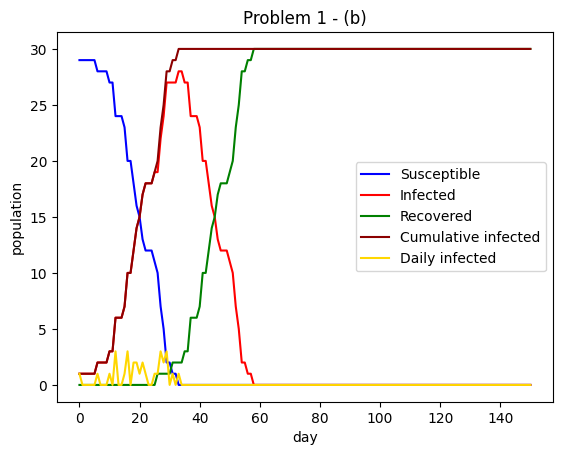
\includegraphics[width=0.5\textwidth ]{Problem1_b_speed3.png}}}
				\subfloat[ \texttt{recovery} = 40]{{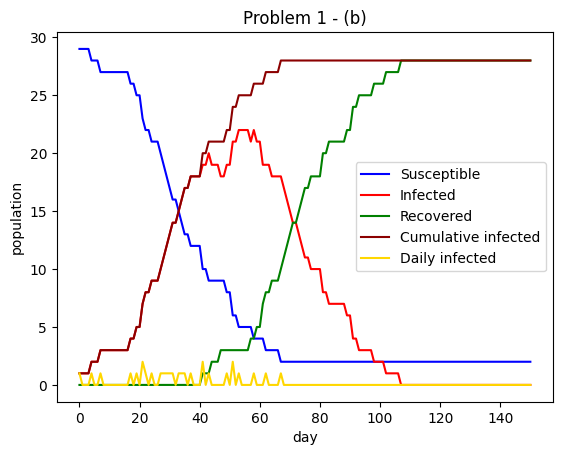
\includegraphics[width=0.5\textwidth ]{Problem1_b_recovery40.png}}}
				\hfill
				\subfloat[\texttt{distance} = 0.06]{{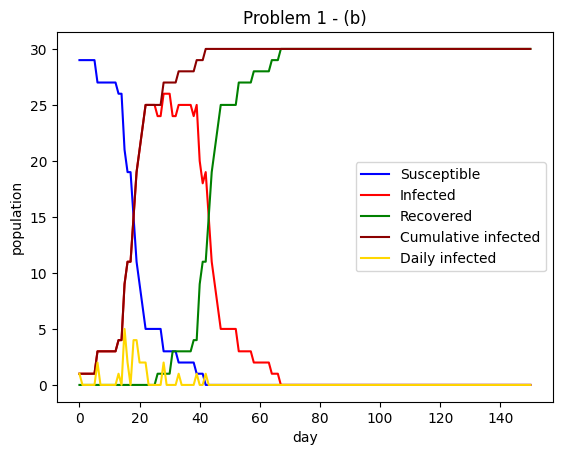
\includegraphics[width=0.5\textwidth ]{Problem1_b_distance6.png}}}
				\subfloat[\texttt{speed} = 0.03, \texttt{recovery} = 40, \texttt{distance} = 0.06]{{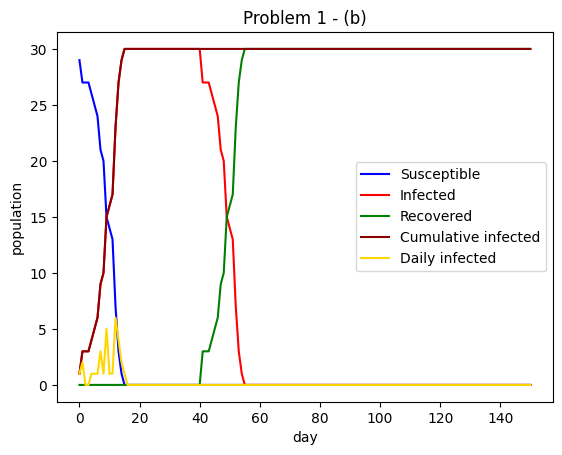
\includegraphics[width=0.5\textwidth ]{Problem1_b_all.png}}}
			\end{figure}
			Differential equation models are based on theoretical formulas. Infection and recovery occur numerically according to the social distance $\beta$ and recovery rate $\gamma$. This is advantageous in explaining the long-term spread trend of infectious diseases, but may not properly reflect local reality.\\
			The particle model takes into account social movement: distance and speed. Therefore, the number of infected and recovered people each day is not consistent. This is advantageous for simulated observations based on reality, but it may be difficult to calculate long-term trends due to the complexity of calculations and various variables.\\
		\end{proof}
		\item 
		\begin{proof} [Solution]
			In model a), since the total number of people is only 30, it is a little difficult to compare the number of daily infections. Nevertheless, the model in a) can be seen as similar to the Seoul and Gyeonggi regions. Compared to other regions, the infection spreads slowly over a long period of time after it begins. On the other hand, there is a big difference from the Daegu and Gyeongbuk regions. This can rather be seen as similar to model b). In the early stages of the spread, the number of infected people increases rapidly. According to our particle model, the \texttt{speed}(social movement distance) and \text{distance}(degree of crowding) of early infected people were high.\\
			Let’s also look at foreign cases. Like the model in a), Rome shows a long-term trend of gradual spread after the initial infection. Italy and Germany increase rapidly in a short period of time, which is similar to the changes in the Daegu and Gyeongbuk regions. Sweden has maintained a consistently low number of infected people despite early infections, perhaps due to good control of variables. However, given that a rapid increase of nearly three times occurred at the end, it appears that it will follow Germany's pattern in the future.\\
		\end{proof}
	\end{enumerate}